\documentclass[12pt, a4paper]{article}

\usepackage[T1]{fontenc}
\usepackage{graphicx}
\usepackage{hyperref}
\usepackage[brazil]{babel}
\usepackage{geometry}
\usepackage{color}
\usepackage{pythonhighlight}
\usepackage[utf8]{inputenc}
\usepackage{indentfirst}
\usepackage{verbatim}
\usepackage{multirow}
\usepackage{booktabs}

\lstset{
	numbers=left,
}

\geometry{
	a4paper,
	left=30mm,
	right=20mm,
	top=30mm,
	bottom=20mm
}

\title{
    \textbf{IESB} \\
    \large Big Data e Inteligência Analítica \\
    \vspace{10cm}
    \textbf{Projeto Integrador em Big Data e Inteligência Analítica}
    \author{Lucas Siqueira Rodrigues}
    \date{}
}

\begin{document}

\begin{titlepage} 
    \maketitle
    \begin{center}
        \vspace{\fill}
        Brasília - DF \\
        Junho de 2025
    \end{center}
\end{titlepage}

\section{Obtenção da base de dados}
\subsection{Introdução}
O trabalho tem como objetivo explorar os dados públicos disponibilizados pela Câmara dos Deputados para analisar e compreender os gastos realizados pelos parlamentares. Para isso, os dados serão obtidos por meio do portal dos dados abertos da câmara\cite{dados_abertos}, armazenados em um banco de dados relacional na nuvem e, posteriormente, analisados.

\subsection{Motivação}
A transparência pública é essencial para garantir a confiança da população nas instituições governamentais. Esse projeto busca realizar um ciclo completo de extração, transformação, armazenamento e análise dos dados de gastos públicos. Além disso, ao construir dashboards, espera-se fornecer ferramentas que possam auxiliar na identificação de possíveis irregularidades e na fiscalização das despesas parlamentares.


\subsection{Script e Banco de Dados}
Para o ano de 2022, a obtenção dos dados por meio da API\cite{dados_abertos} retornou apenas 31 registros.

\begin{python}
import io
import json
import zipfile

import httpx
from tqdm import tqdm

class CamaraAPI:
	def __init__(self) -> None:
		self.base_url = "https://dadosabertos.camara.leg.br/api/v2"
	
	def request(self, endpoint: str) -> dict:
		response = httpx.get(f"{self.base_url}/{endpoint}")
		return response.json()
	
	def get_deputados(self) -> dict:
		return self.request("deputados").get("dados", {})
	
	def get_despesas(self, id_: int, year: int = 2022) -> dict:
		return self.request(f"deputados/{id_}/despesas?ano={year}")

despesas = []

api = CamaraAPI()

deputados = api.get_deputados()
for deputado in tqdm(deputados):
	id_ = deputado["id"]
	despesas_deputado = api.get_despesas(id_=id_, year=2022)
	despesas.extend(despesas_deputado["dados"])

print(len(despesas))  # output: 31
\end{python}

Por isso, apenas para esse ano a coleta de dados foi por meio de um arquivo no formato JSON, que também é fornecido no portal de dados abertos da câmara na aba “Arquivos”.

\begin{figure}[!htbp]
    \centering
    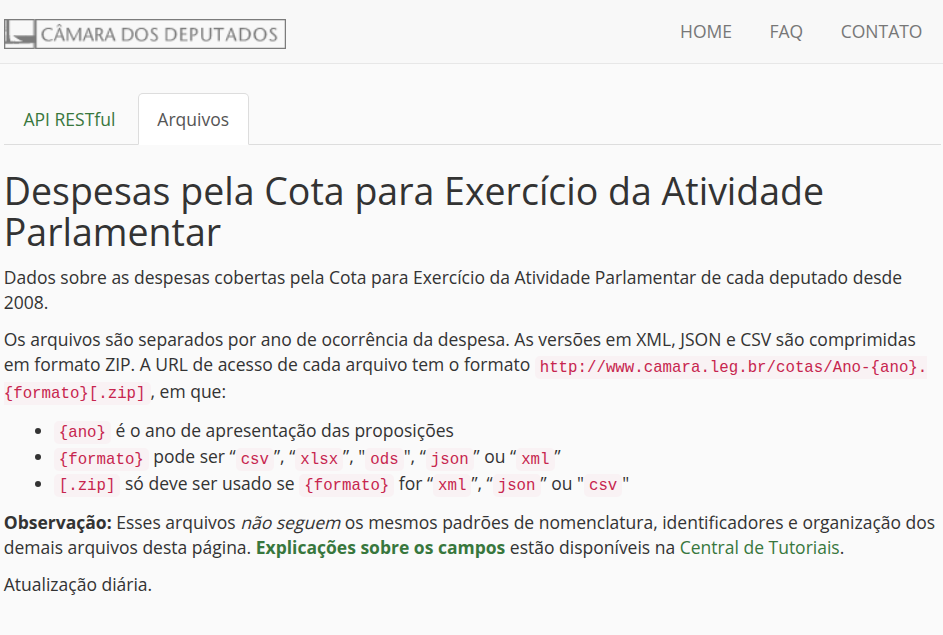
\includegraphics[width=0.8\textwidth]{assets/1_arquivos.png}
    \caption{Coleta de dados por meio da aba de arquivos.}
    \label{fig:arquivo_json}
\end{figure}

Para os anos de 2023 e 2024 a obtenção dos dados foi realizada por meio da API\cite{dados_abertos} da Câmara dos Deputados, explorando dois principais endpoints:
\begin{itemize}
    \item \textbf{/deputados}: Retorna informações gerais sobre os parlamentares, como seus nomes, partidos, estados e e-mails.
    \item \textbf{/deputados/\{id\}/despesas}: Fornece detalhes sobre as despesas realizadas pelos parlamentares, incluindo valores, fornecedores, tipos de despesa e datas, para se ter uma consulta mais completa, devemos adicionar filtros como mês, ano, legislatura, CNPJ ou CPF de um fornecedor, no nosso caso adicionaremos filtros para os anos, ficando com a url: /deputados/\{id\}/despesas?ano=\{ano\}.
\end{itemize}

Para organizar os dados de forma eficiente e integrar os dados obtidos por meio da API e por meio do JSON, foi criado um modelo de banco de dados relacional com tabelas normalizadas para representar as informações de deputados, despesas e fornecedores\cite{dbdiagram}.

\begin{figure}[htbp]
	\centering
	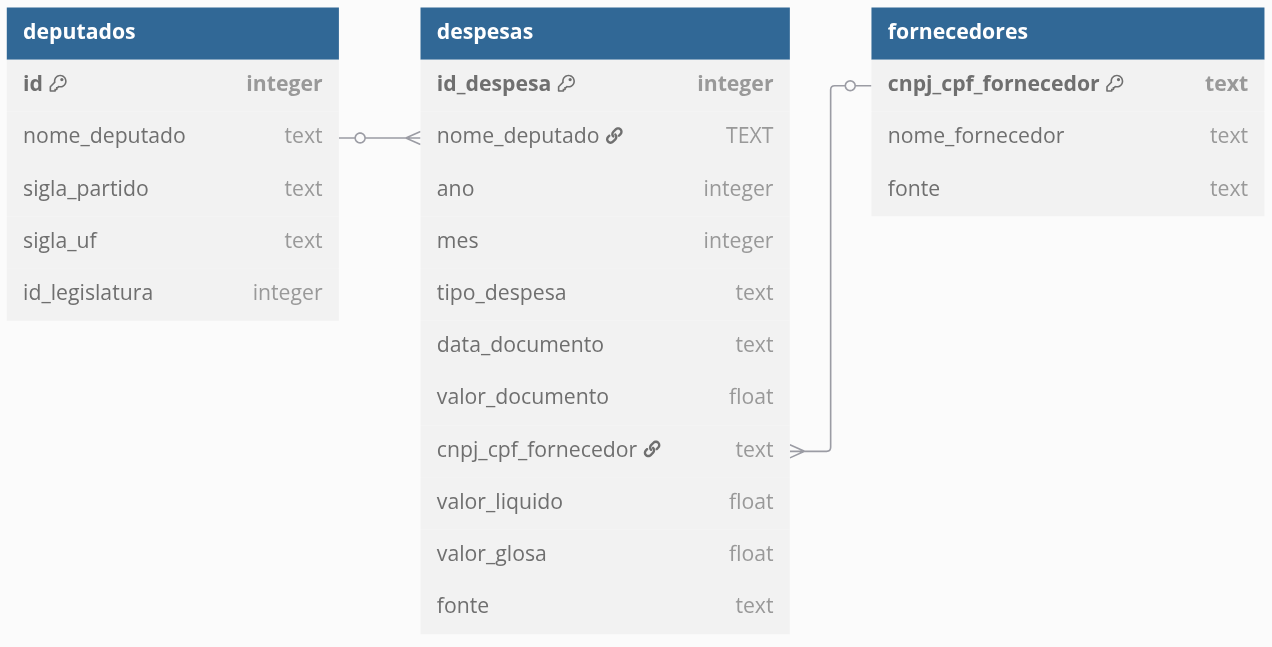
\includegraphics[width=0.8\textwidth]{assets/1_dbdiagram.png}
	\caption{Diagrama relacional.}
	\label{fig:arquivo_json}
\end{figure}
\newpage

Os dados são obtidos e unificados por meio da classe DataService.

\begin{python}
import io
import json
import re
import zipfile

import httpx
from tqdm import tqdm

from data_ingestion.services.log_service import logger


class DataService:
	def __init__(self) -> None:
	self.api_base_url = "https://dadosabertos.camara.leg.br/api/v2"
	
	def get_deputados(self) -> list:
		response = httpx.get(f"{self.api_base_url}/deputados")
		data = response.json().get("dados")
		selected_data = [
			{
				"id": i["id"],
				"nome": i["nome"],
				"sigla_partido": i["siglaPartido"],
				"id_legislatura": i["idLegislatura"],
				"sigla_uf": i["siglaUf"],
			}
			for i in data
			]
	
		return selected_data
	
	def get_data_from_api(self, anos: list[int]) -> tuple[list[dict], list[dict], list[dict]]:
		deputados = self.get_deputados()
		despesas = []
		fornecedores = []
		for ano in anos:
			logger.info(f"Getting data from API for year {ano}")
			for deputado in tqdm(deputados):
				response = httpx.get(f"{self.api_base_url}/deputados/{deputado['id']}/despesas?ano={ano}")
				despesas_deputado = response.json().get("dados")
		
				for item in despesas_deputado:
					despesas.append({
						"nome_deputado": deputado.get("nome"),
						"ano": item.get("ano"),
						"mes": item.get("mes"),
						"tipo_despesa": item.get("tipoDespesa"),
						"data_documento": item.get("dataDocumento"),
						"valor_documento": item.get("valorDocumento"),
						"cnpj_cpf_fornecedor": re.sub(r"[^0-9]", "", item.get("cnpjCpfFornecedor")),
						"valor_liquido": item.get("valorLiquido"),
						"valor_glosa": item.get("valorGlosa"),
						"fonte": "api",
					})
		
					fornecedores.append({
						"nome_fornecedor": item.get("nomeFornecedor"),
						"cnpj_cpf_fornecedor": re.sub(r"[^0-9]", "", item.get("cnpjCpfFornecedor")),
						"fonte": "api",
					})
		
		logger.info(f"Total number of despesas: {len(despesas)}")
		
		return deputados, despesas, fornecedores
	
	@staticmethod
	def get_data_from_url(url: str) -> tuple[list[dict], list[dict], list[dict]]:
		logger.info(f"Getting data from url: {url}")
		response = httpx.get(url=url)
		zip_content = response.content
		
		with zipfile.ZipFile(io.BytesIO(zip_content)) as zip_file:
			with zip_file.open(zip_file.namelist()[0]) as json_file:
				json_content = json_file.read().decode("utf-8")
				json_data = json.loads(json_content).get("dados")
		
		deputados = []
		despesas = []
		fornecedores = []
		
		for item in json_data:
			deputados.append({
				"id": item["numeroDeputadoID"],
				"nome": item["nomeParlamentar"],
				"sigla_partido": item["siglaPartido"],
				"id_legislatura": item["codigoLegislatura"],
				"sigla_uf": item["siglaUF"],
			})
			
			despesas.append({
				"nome_deputado": item.get("nomeParlamentar"),
				"ano": item.get("ano"),
				"mes": item.get("mes"),
				"tipo_despesa": item.get("descricao"),
				"data_documento": item.get("dataEmissao"),
				"valor_documento": item.get("valorDocumento"),
				"cnpj_cpf_fornecedor": re.sub(r"[^0-9]", "", item.get("cnpjCPF")),
				"valor_liquido": item.get("valorLiquido"),
				"valor_glosa": item.get("valorGlosa"),
				"fonte": "url",
			})
			
			fornecedores.append({
				"nome_fornecedor": item.get("fornecedor"),
				"cnpj_cpf_fornecedor": re.sub(r"[^0-9]", "", item.get("cnpjCPF")),
				"fonte": "url",
			})
		
		logger.info(f"Total number of despesas: {len(despesas)}")
		
		return deputados, despesas, fornecedores
\end{python}

A persistência dos dados na base de dados é feita por meio da classe DBService. Ela permite a ingestão dos dados em uma tabela SQLite e MySQL, a tabela do SQLite foi criada e usada apenas para o proprósito de desenvolvimento.

\begin{python}
from sqlalchemy import Column, Float, Integer, String, create_engine, insert
from sqlalchemy.orm import declarative_base, sessionmaker

from data_ingestion.services.log_service import logger

Base = declarative_base()


class Despesas(Base):
	tablename__ = "despesas"
	id = Column(Integer, primary_key=True, autoincrement=True)
	nome_deputado = Column(String(100))
	ano = Column(Integer)
	mes = Column(Integer)
	tipo_despesa = Column(String(100))
	data_documento = Column(String(100))
	valor_documento = Column(Float)
	cnpj_cpf_fornecedor = Column(String(100))
	valor_liquido = Column(Float)
	valor_glosa = Column(Float)
	fonte = Column(String(100))


class Fornecedores(Base):
	tablename__ = "fornecedores"
	id = Column(Integer, primary_key=True, autoincrement=True)
	nome_fornecedor = Column(String(100))
	cnpj_cpf_fornecedor = Column(String(100), unique=True)
	fonte = Column(String(100))


class Deputados(Base):
	tablename__ = "deputados"
	id = Column(Integer, primary_key=True)
	nome = Column(String(100), unique=True)
	sigla_partido = Column(String(100))
	id_legislatura = Column(Integer)
	sigla_uf = Column(String(100))


class DBService:
	def __init__(
		self,
		local: bool = False,
		user: str | None = None,
		password: str | None = None,
		host: str | None = None,
		port: int | None = None,
		dbname: str | None = None,
	) -> None:
		if local:
			self.engine = create_engine("sqlite:///database.db")
			self.dialect = "sqlite"
		else:
			self.engine = create_engine(f"mysql+pymysql://{user}:{password}@{host}:{port}/{dbname}", pool_recycle=3600)
			self.dialect = "mysql"

		self.Session = sessionmaker(bind=self.engine)
	
	def insert_data(self, deputados: list, despesas: list, fornecedores: list) -> None:
		Base.metadata.create_all(self.engine)
		session = self.Session()
		
		try:
			logger.info("Inserindo deputados")
			if deputados:
				stmt = insert(Deputados)
				if self.dialect == "sqlite":
					stmt = stmt.prefix_with("OR IGNORE")
				elif self.dialect == "mysql":
					stmt = stmt.prefix_with("IGNORE")
				session.execute(stmt, deputados)
			
			logger.info("Inserindo fornecedores")
			if fornecedores:
				stmt = insert(Fornecedores)
				if self.dialect == "sqlite":
					stmt = stmt.prefix_with("OR IGNORE")
				elif self.dialect == "mysql":
					stmt = stmt.prefix_with("IGNORE")
				session.execute(stmt, fornecedores)
			
			logger.info("Inserindo despesas")
			if despesas:
				stmt = insert(Despesas)
				if self.dialect == "sqlite":
					stmt = stmt.prefix_with("OR IGNORE")
				elif self.dialect == "mysql":
					stmt = stmt.prefix_with("IGNORE")
				session.execute(stmt, despesas)
			
			session.commit()
		finally:
			session.close()
\end{python}

E por fim, temos a função main(), que realiza todo o ciclo de extração, transformação e carregamento dos dados.

\begin{python}
import os

from dotenv import load_dotenv

from data_ingestion.services.data_service import DataService
from data_ingestion.services.db_service import DBService

_ = load_dotenv()


def main() -> None:
	url = "https://www.camara.leg.br/cotas/Ano-2022.json.zip"
	anos = [2023, 2024]
	
	data_service = DataService()
	api_deputados, api_despesas, api_fornecedores = data_service.get_data_from_api(anos=anos)
	url_deputados, url_despesas, url_fornecedores = data_service.get_data_from_url(url=url)
	
	deputados = [*api_deputados, *url_deputados]
	despesas = [*api_despesas, *url_despesas]
	fornecedores = [*api_fornecedores, *url_fornecedores]
	
	db_service = DBService(
		user=os.environ["DB_USER"],
		password=os.environ["DB_PASSWORD"],
		host=os.environ["DB_HOST"],
		port=int(os.environ["DB_PORT"]),
		dbname=os.environ["DB_NAME"],
	)
	db_service.insert_data(deputados=deputados, despesas=despesas, fornecedores=fornecedores)


if __name__ == "__main__":
	main()
\end{python}

O programa, ao ser executado, faz a extração, transformação e carga de 223.982 registros de despesas dos anos de 2022, 2023 e 2024.

Logo após serem obtidos, os dados são inseridos em um banco de dados MySQL, que foi criado usando o serviço Amazon RDS (Relational Database Service).

\begin{figure}[!htbp]
    \centering
    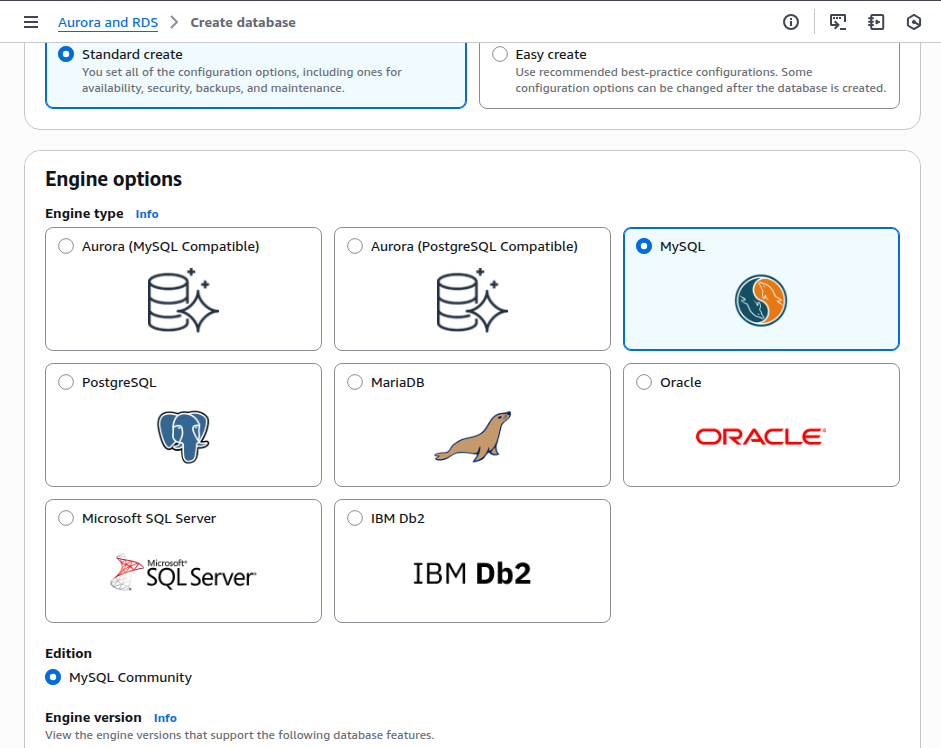
\includegraphics[width=0.8\textwidth]{assets/1_criacao.png}
    \caption{Criação do MySQL na AWS.}
    \label{fig:criacao_mysql}
\end{figure}
\newpage

Após a base de dados ser criada, podemos nos conectar a ela usando o DBeaver\cite{dbeaver}.

\begin{figure}[!htbp]
    \centering
    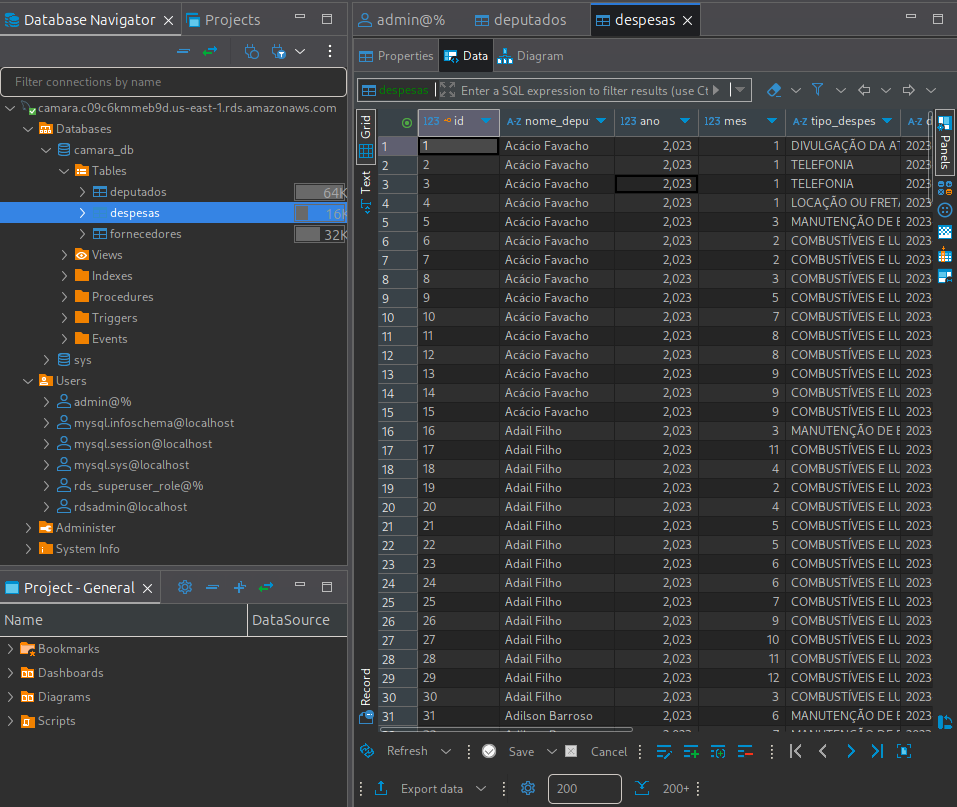
\includegraphics[width=0.8\textwidth]{assets/1_dbeaver.png}
    \caption{Base de dados conectada no DBeaver.}
    \label{fig:db conexão}
\end{figure}

Todo o código relacionado ao projeto está no Github\cite{github_repo}.

\subsection{Considerações finais}

A combinação de tecnologias como Python, AWS e MySQL foi fundamental para realizar as etapas de extração, transformação e carregamento dos dados. A API da Câmara revelou-se limitada em relação à quantidade de dados retornados para o ano de 2022, mas a extração dos dados do JSON da aba Arquivos permitiu superar essa restrição e criar uma base robusta com uma quantidade considerável de dados.

\section{Relatório Analítico}

\subsection{Introdução}

A análise de dados públicos desempenha um papel crucial na promoção da transparência governamental e no combate a irregularidades. Utilizando o Streamlit para a criação de dashboards, é possível transformar grandes volumes de dados em informações compreensíveis e acessíveis para a população e órgãos de fiscalização.

\subsection{Demonstração}

O Streamlit foi integrado ao banco de dados MySQL, permitindo consultas em tempo real e construção de dashboards dinâmicos.

Na nossa base de dados foram construídas 3 tabelas, e para facilitar o processo de construção de gráficos uma query foi feita realizando o join das tabelas.

\begin{verbatim}
SELECT
	despesas.nome_deputado,
	despesas.ano,
	despesas.mes,
	despesas.tipo_despesa,
	despesas.valor_documento,
	despesas.cnpj_cpf_fornecedor,
	deputados.sigla_partido,
	deputados.id_legislatura,
	deputados.sigla_uf,
	fornecedores.nome_fornecedor
FROM
	despesas
LEFT JOIN
	deputados on despesas.nome_deputado = deputados.nome
LEFT JOIN
	fornecedores ON despesas.cnpj_cpf_fornecedor = fornecedores.cnpj_cpf_fornecedor;
\end{verbatim}

A partir dos dados recuperados da base de dados criamos um dataframe do Pandas\cite{Pandas}, nele podemos aplicar filtros e realizar agrupamentos nos dados para extrair informações e criar gráficos.

\begin{python}
grouped_df = df[["tipo_despesa", "valor_documento"]].groupby("tipo_despesa").sum()
st.bar_chart(grouped_df, horizontal=True, x_label="Valor total em R$")
\end{python}

\begin{figure}[!htbp]
	\centering
	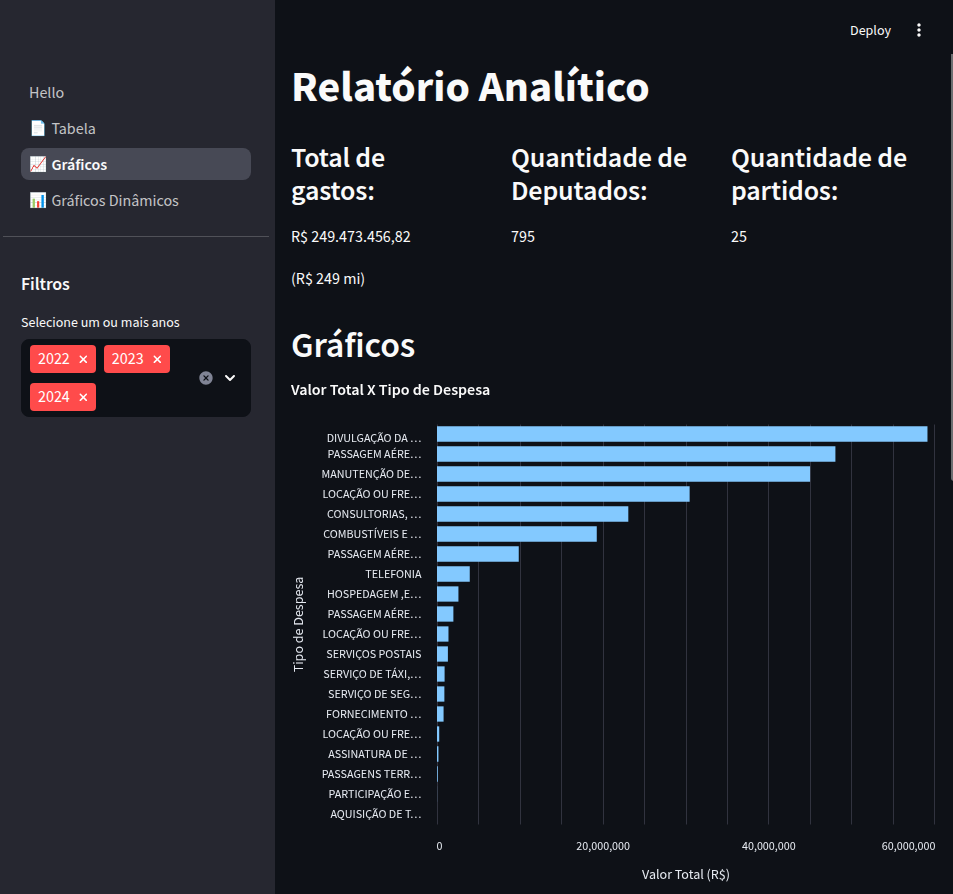
\includegraphics[width=0.8\textwidth]{assets/2_plot1.png}
	\caption{Gráfico mostrando a quantidade de gastos por tipo de despesa.}
	\label{fig:criacao_postgresql}
\end{figure}

\subsection{Relatórios e tabelas}

Aqui podemos analisar o gastos dos anos de 2022, 2023 e 2024 de forma combinada ou isolada. Temos que o total de gastos são:

\begin{table}[htbp]
	\centering
	\begin{tabular}{llll}
		\toprule
		Ano & Total de Gastos & Quantidade de Deputados \\
		\midrule
		Combinados & R\$ 249 mi & 795 \\
		2022 & R\$ 221 mi & 572 \\
		2023 & R\$ 14 mi & 494 \\
		2024 & R\$ 14 mi & 496 \\
		\bottomrule
	\end{tabular}
	\caption{Resumo de gastos.}
	\label{tab:minhatabela1}
\end{table}

Para os anos combinados, temos que DIVULGAÇÃO DA ATIVIDADE PARLAMENTAR foi a categoria de gastos com o maior valor, seguido de PASSAGEM AÉREA - SIGEPA e MANUTENÇÃO DE ESCRITÓRIO DE APOIO À ATIVIDADE PARLAMENTAR.

\begin{figure}[!htbp]
	\centering
	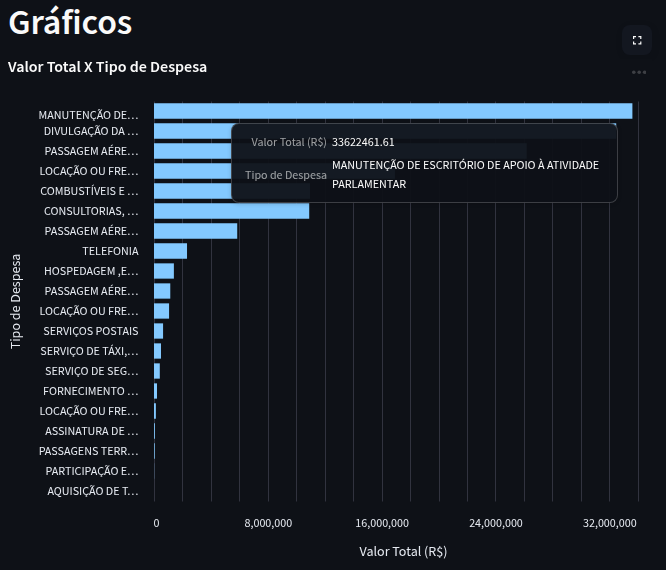
\includegraphics[width=0.8\textwidth]{assets/2_plot2.png}
	\caption{Valor dos gastos por tipo de despesa.}
	\label{fig:criacao_postgresql}
\end{figure}
\newpage

Giacobo foi o parlamentar com a maior quantidade de gastos, totalizando R\$ 1.289.809,76 em gastos, seguido por Silas Câmara com R\$ 1.177.321,09 e Gustinho Ribeiro com R\$ 1.061.509,11.

\begin{figure}[!htbp]
	\centering
	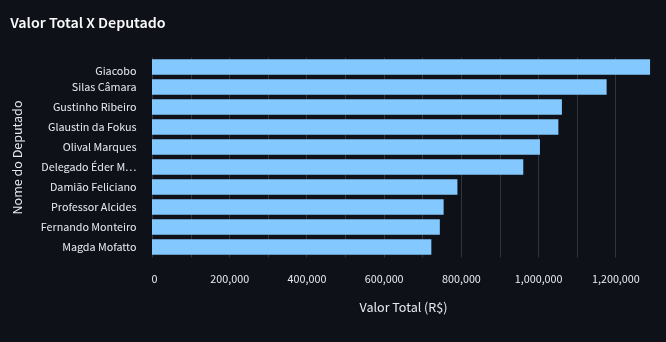
\includegraphics[width=0.8\textwidth]{assets/2_plot3.png}
	\caption{Valor dos gastos por deputado.}
	\label{fig:criacao_postgresql}
\end{figure}

Com relação aos fornecedores, as 3 maiores são empresas de companhias aéreas. A TAM foi disparadamente a maior, com gastos totalizando R\$ 48 milhões, seguida por Latam Linhas Aéreas com R\$ 5 milhões e Gol Linhas Aéreas com quase R\$ 4 milhões.

\begin{figure}[!htbp]
	\centering
	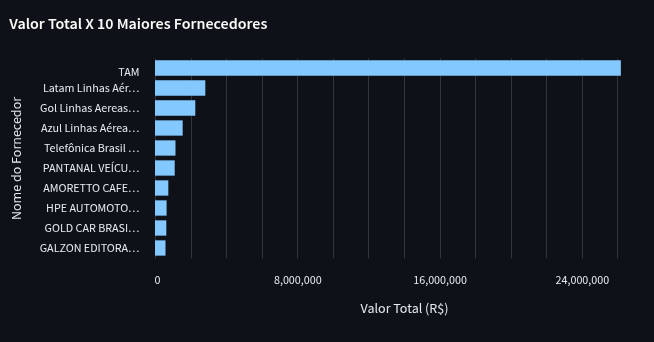
\includegraphics[width=0.8\textwidth]{assets/2_plot4.png}
	\caption{Valor dos gastos por fornecedor.}
	\label{fig:criacao_postgresql}
\end{figure}

Usando o streamlit também podemos criar gráficos dinâmicos para analisar os dados separados por categorias, assim podemos selecionar a variável de interesse e a função de agregação, para assim poder analisar o total de gastos, média, valor máximo e muito mais.

\begin{figure}[!htbp]
	\centering
	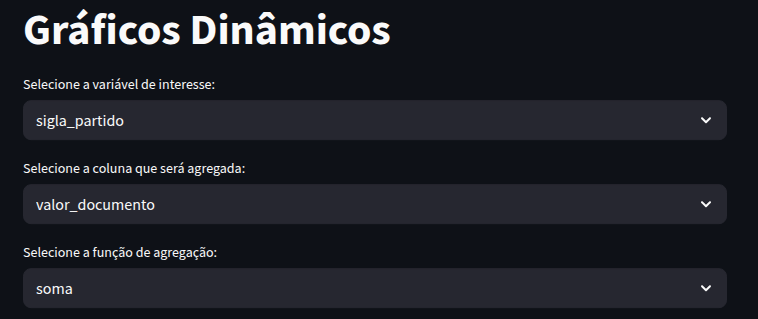
\includegraphics[width=0.8\textwidth]{assets/2_plot5.png}
	\caption{Gráfico dinâmico.}
	\label{fig:criacao_postgresql}
\end{figure}
\newpage

Ao selecionar a categoria sigla\_partido, podemos ver que os partidos com o maior número de gastos foi o PL com R\$ 34 milhões, seguido pelo PP com R\$ 28 milhões e o PT com R\$ 27 milhões.

\begin{figure}[!htbp]
	\centering
	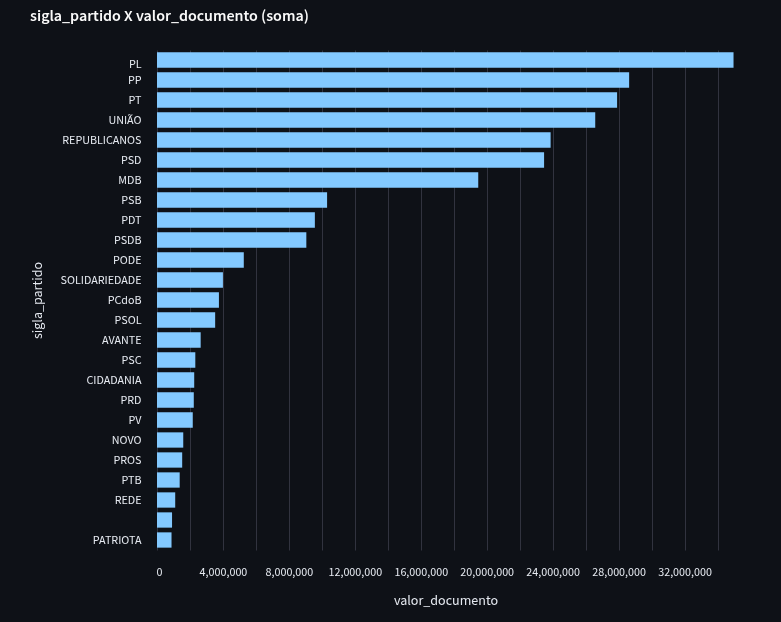
\includegraphics[width=0.8\textwidth]{assets/2_plot6.png}
	\caption{Valor dos gastos por partido.}
	\label{fig:criacao_postgresql}
\end{figure}

Podemos filtrar os gastos por UF, calculando o valor total dos gastos nesse estado.

\begin{figure}[!htbp]
	\centering
	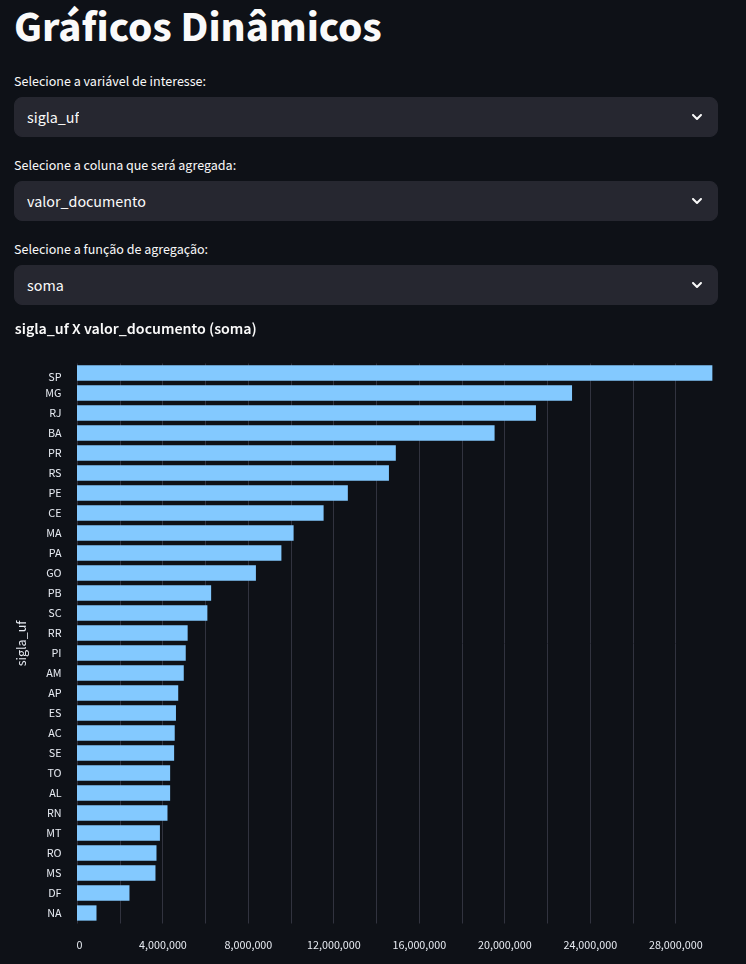
\includegraphics[width=0.8\textwidth]{assets/2_plot7.png}
	\caption{Valor dos gastos por UF.}
	\label{fig:criacao_postgresql}
\end{figure}
\newpage

Trocando a função de agregação, podemos obter outras informações como a média dos gastos por UF.

\begin{figure}[!htbp]
	\centering
	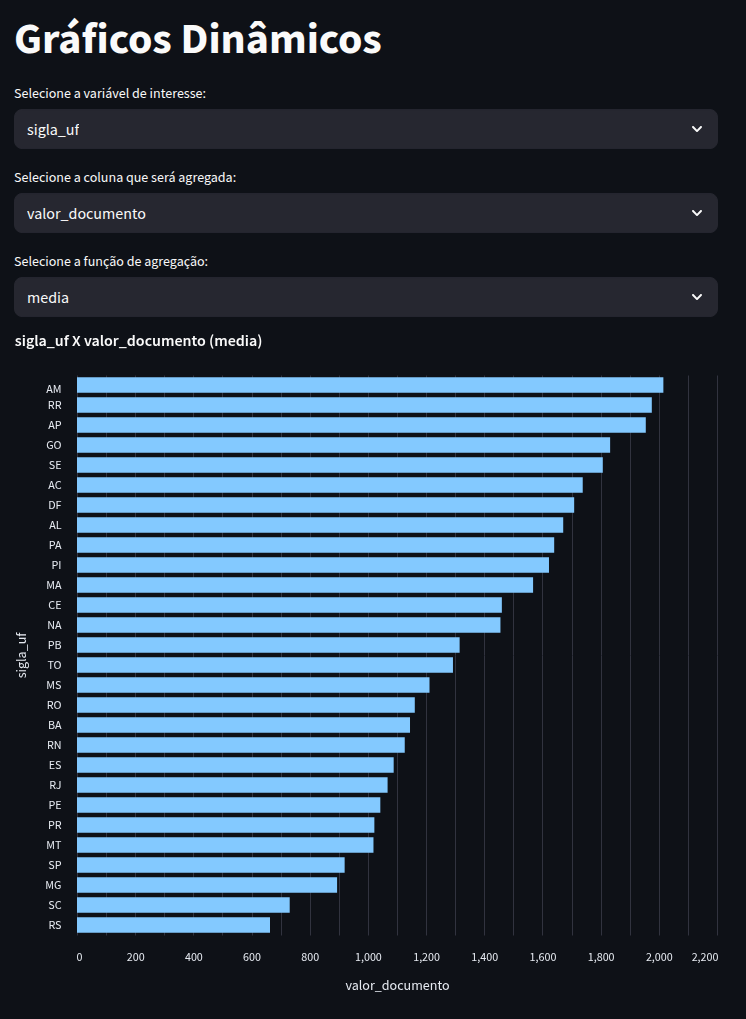
\includegraphics[width=0.8\textwidth]{assets/2_plot8.png}
	\caption{Valor médio dos gastos por UF.}
	\label{fig:criacao_postgresql}
\end{figure}

Outra informação é a tendência de gastos mensais, aqui temos a tendência para os anos 2022, 2023 e 2024, mas como para o ano de 2022 temos uma quantidade bem maior de gastos, fica um pouco difícil analisar, por isso podemos selecionar os anos na barra lateral para então analisar cada ano individualmente.

\begin{figure}[!htbp]
	\centering
	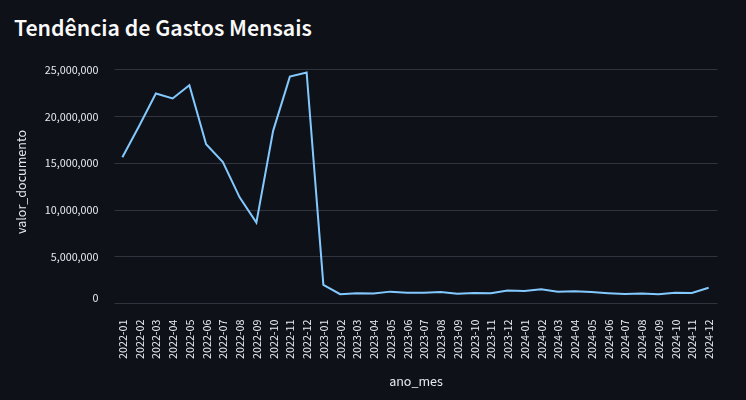
\includegraphics[width=0.8\textwidth]{assets/2_plot9.png}
	\caption{Tendência de gastos para os anos de 2022, 2023 e 2024.}
	\label{fig:tendencia de gastos}
\end{figure}

\newpage

\begin{figure}[!htbp]
	\centering
	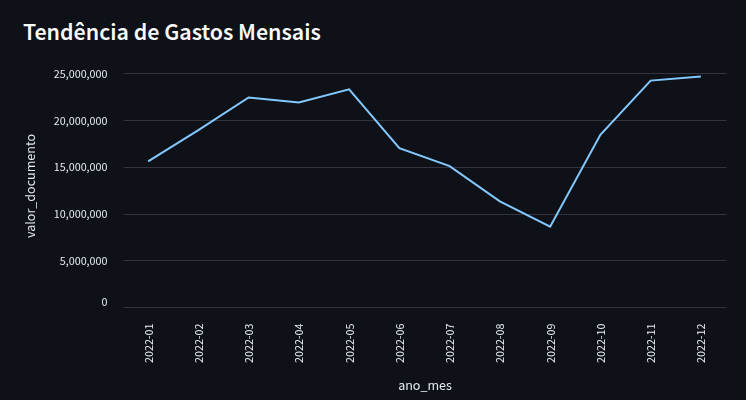
\includegraphics[width=0.8\textwidth]{assets/2_plot10.png}
	\caption{Tendência de gastos para o ano de 2022.}
	\label{fig:tendencia de gastos}
\end{figure}
\newpage

\begin{figure}[!htbp]
	\centering
	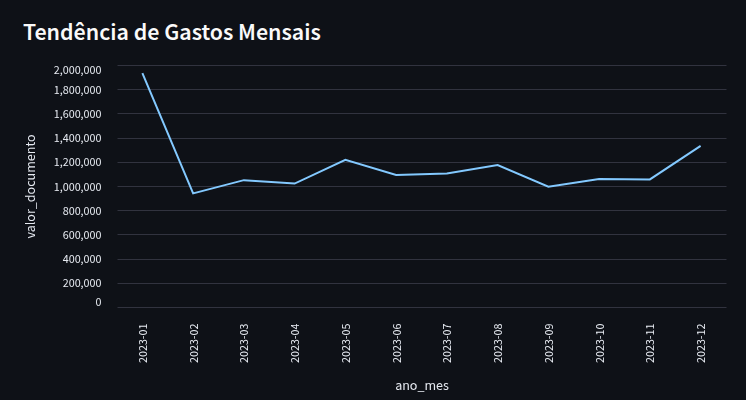
\includegraphics[width=0.8\textwidth]{assets/2_plot11.png}
	\caption{Tendência de gastos para o ano de 2023.}
	\label{fig:tendencia de gastos}
\end{figure}

\begin{figure}[!htbp]
	\centering
	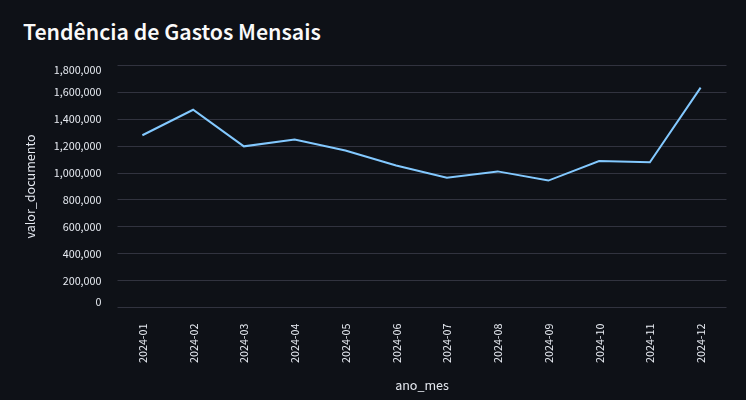
\includegraphics[width=0.8\textwidth]{assets/2_plot12.png}
	\caption{Tendência de gastos para o ano de 2024.}
	\label{fig:tendencia de gastos}
\end{figure}

\subsection{Considerações finais}

O Streamlit é uma ferramenta robusta para análise de dados, permitindo a criação de gráficos interativos que facilitam a compreensão e a extração de insights valiosos. Diferente de plataformas de BI como o Power BI, o Streamlit oferece maior controle e personalização sobre suas visualizações, embora exija conhecimento em programação e um tempo de desenvolvimento inicial maior.

\section{Machine Learning}
\subsection{Introdução}

Machine Learning (Aprendizado de Máquina) é um campo da inteligência artificial que permite aos sistemas aprender com dados, identificar padrões, tomar decisões e fazer predições futuras com mínima intervenção humana. Sua aplicação vai desde a detecção de anomalias e o reconhecimento de padrões em grandes volumes de dados até a otimização de processos e a personalização de experiências. É uma ferramenta poderosa para transformar dados brutos em insights acionáveis.

\subsection{Dicionário de dados}

No contexto do nosso projeto, as seguintes variáveis são selecionadas para a construção do modelo de machine learning:

\begin{itemize}
	\item \textbf{nome\_deputado}: Nome completo do deputado.
	\item \textbf{ano}: Ano em que a despesa foi realizada.
	\item \textbf{mes}: Mês em que a despesa foi realizada.
	\item \textbf{tipo\_despesa}: Categoria da despesa, como "DIVULGAÇÃO DA ATIVIDADE PARLAMENTAR"\ ou  "PASSAGEM AÉREA - SIGEPA".
	\item \textbf{valor\_documento}: Valor da despesa conforme registrado no documento.
	\item \textbf{nome\_fornecedor}: Nome completo do fornecedor do bem ou serviço.
	\item \textbf{sigla\_partido}: Sigla do partido político ao qual o deputado é afiliado.
	\item \textbf{sigla\_uf}: Sigla da Unidade Federativa (estado) pela qual o deputado foi eleito.
\end{itemize}

Com o propósito de criar um modelo de identificação de anomalias nos dados, utilizamos o algoritmo Isolation Forest\cite{Scikit-Learn}.

O Isolation Forest é um algoritmo de Machine Learning não supervisionado amplamente utilizado para detecção de anomalias. Diferente de outros métodos que tentam "encontrar" a normalidade para depois identificar o que é diferente, o Isolation Forest adota uma abordagem mais direta, ele isola as anomalias. Ele funciona da seguinte forma\cite{isolation-forest}:

\begin{enumerate}
	\item \textbf{Construção de Árvores Aleatórias}: O algoritmo constrói uma floresta de árvores de decisão. Para cada árvore, ele seleciona aleatoriamente um atributo e, em seguida, seleciona aleatoriamente um ponto de divisão dentro do intervalo de valores desse atributo.
	\item \textbf{Isolamento de Pontos}: Esse processo de divisão continua até que cada ponto de dado esteja isolado ou um limite de profundidade da árvore seja atingido.
	\item \textbf{Identificação de Anomalias}: O princípio é que as anomalias, por serem pontos mais raros e diferentes, geralmente exigem menos divisões para serem isoladas nas árvores. Pontos normais, por outro lado, são mais densos e requerem mais divisões para serem separados uns dos outros.
\end{enumerate}

Podemos transformar os dados em um dataframe do Pandas\cite{Pandas}, e usá-lo para criar um modelo usando a classe IsolatioForest presente no Scikit-Learn\cite{Scikit-Learn}.

O pré-processamento dos dados é etapa crucial para criar bons modelos de machine learning, iniciaremos essa análise usando a biblioteca missingno para encontrar os valores ausentes no nosso dataset.

\begin{python}
msno.matrix(df, figsize=(12, 5), fontsize=12)

import missingno as msno
\end{python}

Podemos ver que não há nenhuma linha com dado faltante no nosso dataset, por isso a parte de inputação de dados ou remoção de linhas com valores nulos não será necessária.

\begin{figure}[!htbp]
	\centering
	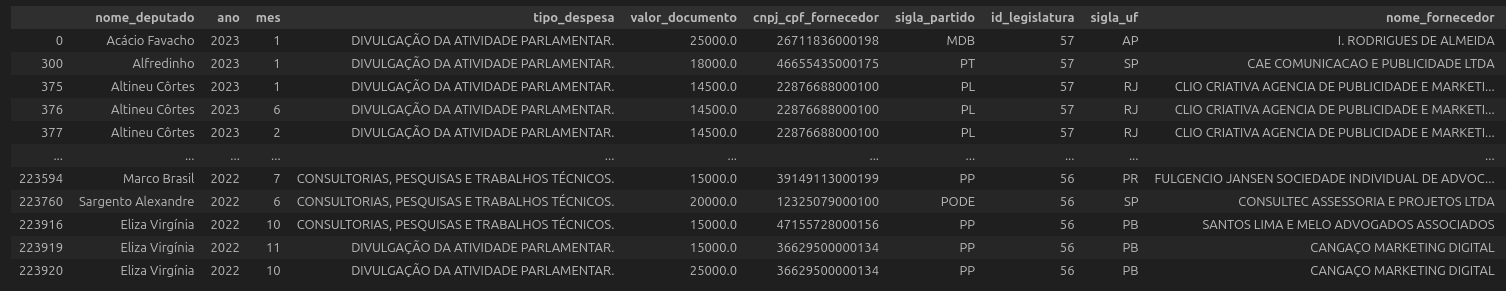
\includegraphics[width=0.8\textwidth]{assets/3_plot1.png}
	\caption{Dados faltantes.}
	\label{fig:dados faltantes}
\end{figure}

Logo após podemos selecionar as features e usar o Label Encoder, com ele convertemos variáveis categóricas em numéricas para que o nosso modelo de machine learning possa computar.

\begin{python}
le_df = df[
	[
		"nome_deputado",
		"ano",
		"mes",
		"tipo_despesa",
		"valor_documento",
		"sigla_partido",
		"sigla_uf",
		"nome_fornecedor",
	]
]

for col in le_df.select_dtypes(include=["object"]).columns:
	label_encoder = LabelEncoder()
	le_df[col] = label_encoder.fit_transform(le_df[col].astype(str))
\end{python}

E por fim temos o nosso dataframe após o Label Encoder.

\begin{figure}[!htbp]
	\centering
	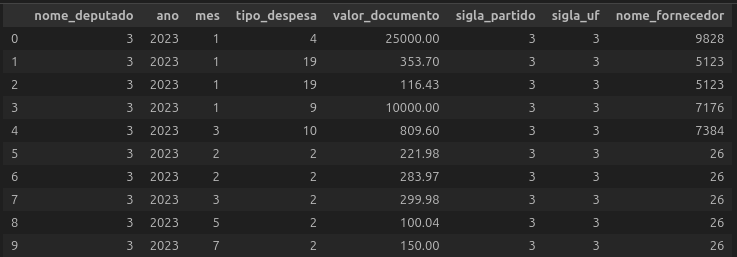
\includegraphics[width=0.8\textwidth]{assets/3_plot2.png}
	\caption{Label Encoder.}
	\label{fig:label encoder}
\end{figure}
\newpage

Após o pré-processamento dos dados podemos dar início ao processo de construção, treinamento e inferência do nosso modelo.

\begin{python}
n_estimators = 100
contamination = 0.01
sample_size = 256	

model = IsolationForest(
	n_estimators=n_estimators,
	contamination=contamination,
	max_samples=sample_size,
	random_state=42
)
model.fit(df)

df["anomaly"] = model.predict(le_df)

# -1 para anomalias, 1 para dados normais
anomalies = df[df["anomaly"] == -1]
\end{python}

E então, temos 2240 anomalias no dataframe contendo 223982 registros, isso representa 1.0000803636006466\% dos registros.

Aqui temos alguns exemplos de dados que foram detectados como anomalias.

\begin{figure}[!htbp]
	\centering
	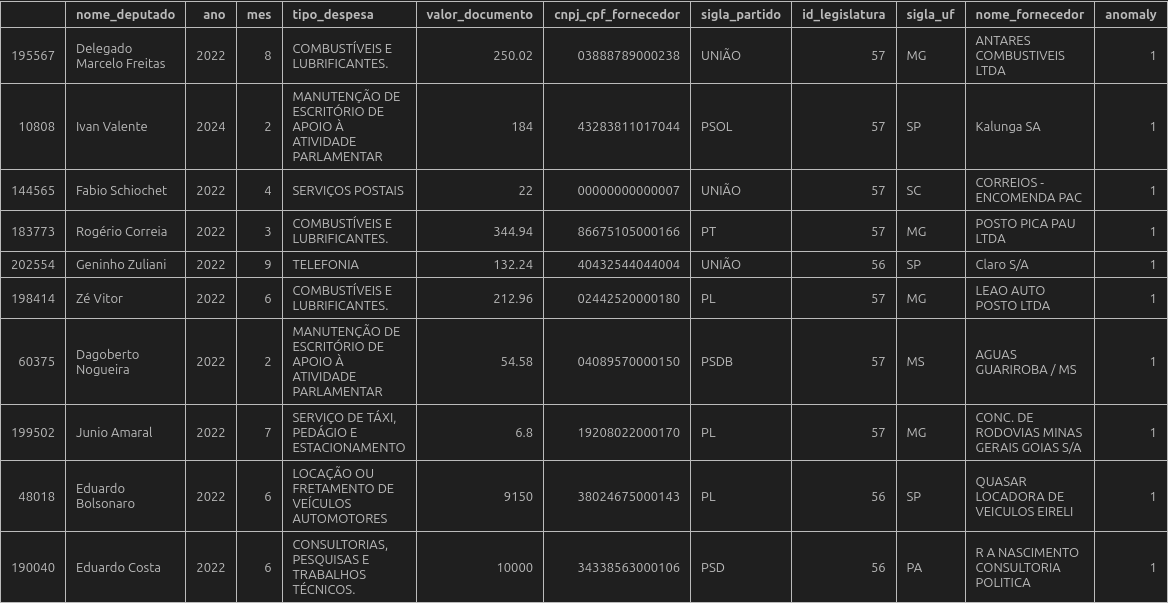
\includegraphics[width=0.8\textwidth]{assets/3_plot3.png}
	\caption{Anomalias nos gastos.}
	\label{fig:anomalias}
\end{figure}

\subsection{Considerações finais}

Para identificar comportamentos ou eventos incomuns que se desviam do padrão em grandes volumes de dados, o Isolation Forest é uma escolha excepcionalmente robusta. Essa ferramenta se mostra muito eficaz na detecção de problemas em gastos e como suporte crucial em auditorias, ajudando a detectar o que realmente importa.

\section{Vídeo}
O vídeo de 10 minutos mostrando todo o projeto foi gravado e disponibilizado por meio do google drive através do link: \href{https://drive.google.com/file/d/14FIFpgSWjTtZ3jbXWYxiaxWnMd5L5SLw/view?usp=sharing}{https://drive.google.com/file/d/14FIFpgSWjTtZ3jbXWYxiaxWnMd5L5SLw/view?usp=sharing}.

\newpage
\begin{thebibliography}{9}
    \bibitem{dados_abertos} Portal de Dados Abertos da Câmara dos Deputados: 
    \href{https://dadosabertos.camara.leg.br/swagger/api.html}{https://dadosabertos.camara.leg.br/swagger/api.html}

    \bibitem{dbdiagram} dbdiagram: 
    \href{https://dbdiagram.io/}{https://dbdiagram.io/}
    
    \bibitem{dbeaver} DBeaver: 
    \href{https://dbeaver.io/}{https://dbeaver.io/}

    \bibitem{github_repo} Repositório do Projeto no Github: 
    \href{https://github.com/lucassiro/pi}{https://github.com/lucassiro/pi}
    
    \bibitem{Pandas} Pandas: 
    \href{https://pandas.pydata.org/}{https://pandas.pydata.org/}
    
    \bibitem{Scikit-Learn} Isolation Forest no Scikit-Learn: 
    \href{https://scikit-learn.org/stable/modules/generated/sklearn.ensemble.IsolationForest.html}{https://scikit-learn.org/stable/modules/generated/sklearn.ensemble.IsolationForest.html}
    
    \bibitem{isolation-forest} Guia da floresta de isolamento: Explicação e implementação em Python: 
    \href{https://www.datacamp.com/pt/tutorial/isolation-forest}{https://www.datacamp.com/pt/tutorial/isolation-forest}
    
    \bibitem{video} Vídeo do projeto: 
    \href{https://drive.google.com/file/d/14FIFpgSWjTtZ3jbXWYxiaxWnMd5L5SLw/view?usp=sharing}{https://drive.google.com/file/d/14FIFpgSWjTtZ3jbXWYxiaxWnMd5L5SLw/view?usp=sharing}
\end{thebibliography}

\end{document}